\subsection{Molten Salt Reactors}

\begin{frame}
\frametitle{MSR (Molten Salt Reactor) types}
\begin{overlayarea}{\linewidth}{20\baselineskip}
\begin{block}{Stationary Fuel}<1-4>
	\begin{enumerate}
		\item Graphite block with TRISO fuel, clean salt works as 
		coolant (Fluoride-Salt-Cooled High-Temperature 
		Reactor (FHR))
		\item Plate Fuel: hexagonal fuel assembly is similar in shape to a typical sodium-cooled reactor
		\item Fuel Inside Radial Moderator (FIRM)
		\item Liquid fuel salt inside fuel rods cooled by clean salt 
		(Moltex Stable Salt Reactor)
	\end{enumerate}
\end{block}

\begin{block}{Mobile Fuel}<2-4>
	\begin{enumerate}
		\item<2-4> Mobile solid fuel elements (pebbles) cooled by 
		clean salt (PB-FHR)
		\item<3-4> Non-circulating liquid fuel salt (TerraPower \gls{MCFR}) 
		\item<4> \textbf{Circulating liquid fuel salt} which also works 
		as coolant (\gls{MSBR}, \gls{MSFR})
	\end{enumerate}
\end{block}
\end{overlayarea}
\end{frame}

\begin{frame}
\frametitle{Stationary and Mobile Solid fuel}
\vspace*{-0.1in}
\begin{figure}[t]
	\hspace*{-0.35in}
	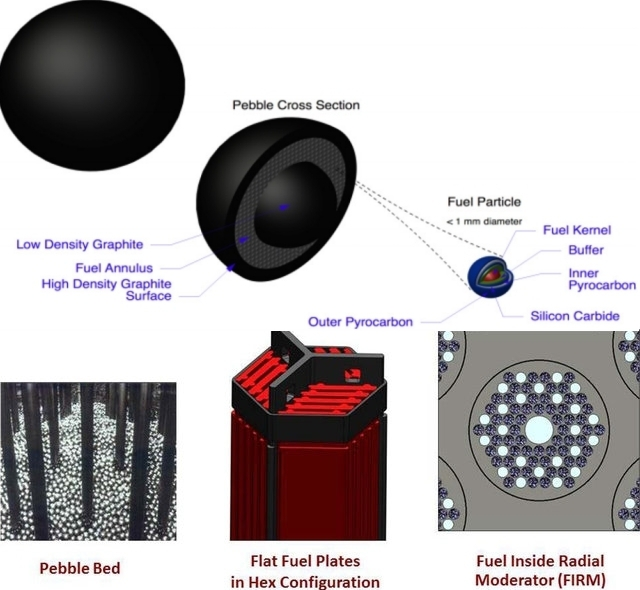
\includegraphics[height=0.63\textwidth]{./images/solid_fuel.jpg}
	\caption{TRISO fuel particle (top) and FHR fuel designs (bottom). Source \cite{forsberg_basis_2016-1}.}
\end{figure}   
\end{frame}

\begin{frame}
\frametitle{Mobile, Non-Circulating, Liquid Fuel}
\begin{figure}[t]
\vspace*{-0.1in}
\hspace*{-0.35in}
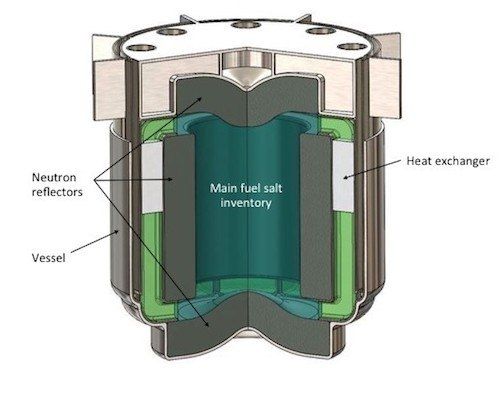
\includegraphics[height=0.6\textwidth]{./images/mcfr-crossection.jpg}
\caption{The TerraPower MCFR is an example of reactor design with \textbf{liquid, mobile, non-circulating} chloride salt fuel. Source \cite{doene_southern_2018}.}
\end{figure}   

\end{frame}

\begin{frame}
\frametitle{Mobile, Circulating, Liquid Fuel}
\begin{figure}[t]
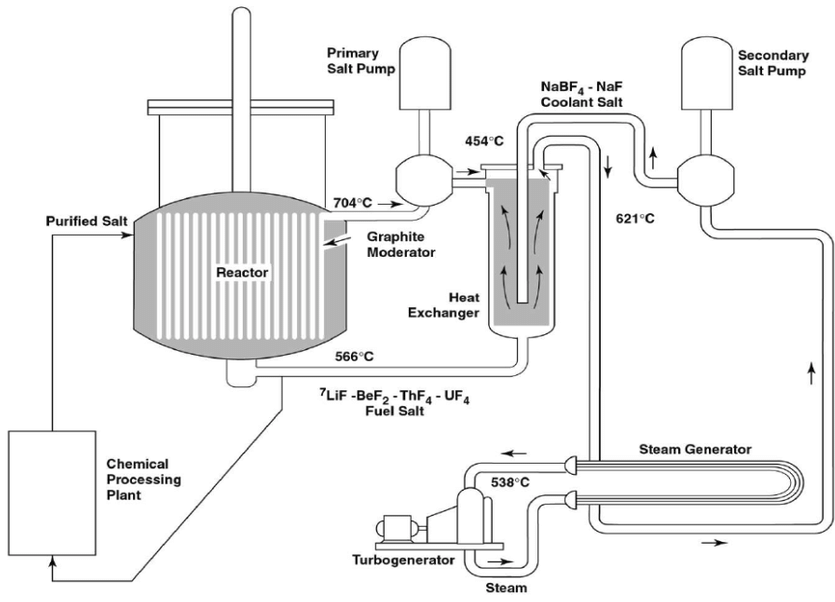
\includegraphics[height=0.58\textwidth]{./images/msbr_scheme.png}
\caption{The \gls{MSBR} is an example of reactor design with \textbf{liquid, mobile, circulating} fluoride salt fuel \cite{rosenthal_molten-salt_1970}.}
\end{figure}   

\end{frame}

\subsection{Motivation}


\begin{frame}
\frametitle{Why Molten Salt Reactors with circulating fuel?}
\begin{block}{Liquid-fueled \glsfirst{MSR} 
		designs have following \textbf{potential} advantages:}
	\begin{enumerate}
		\itemsep1em
		\item High coolant temperature (600-750$^{\circ}$C) 
		$\Rightarrow$ potentially high thermal efficiency, process 
		heat for chemical industry
		\item Fuel diversity ($^{235}$U, $^{233}$U, Thorium, U/Pu)
		\item Strong negative temperature feedback of liquid fuel
		\item Passive safety $\Rightarrow$ fuel drains into tanks 
		in emergency
		\item High fuel utilization $\Rightarrow$ less nuclear 
		waste generated
		\item<2> \textbf{On-line (continuous) fuel reprocessing and refueling}
	\end{enumerate}
\end{block}

\end{frame}


\begin{frame}
  \frametitle{Challenges in \gls{MSR} Simulation}
                  \vspace*{-0.05in}
               \begin{enumerate}
                \item Contemporary burnup codes cannot treat fuel movement
                \item Neutron precursor location is hard to estimate
                \item Operational and safety parameters change during reactor operation
                \item Power generation strongly depends on fuel temperature and vica versa
               \end{enumerate}

           \begin{figure}[t]
                \vspace*{-0.05in}
			\hspace*{-0.2in}
                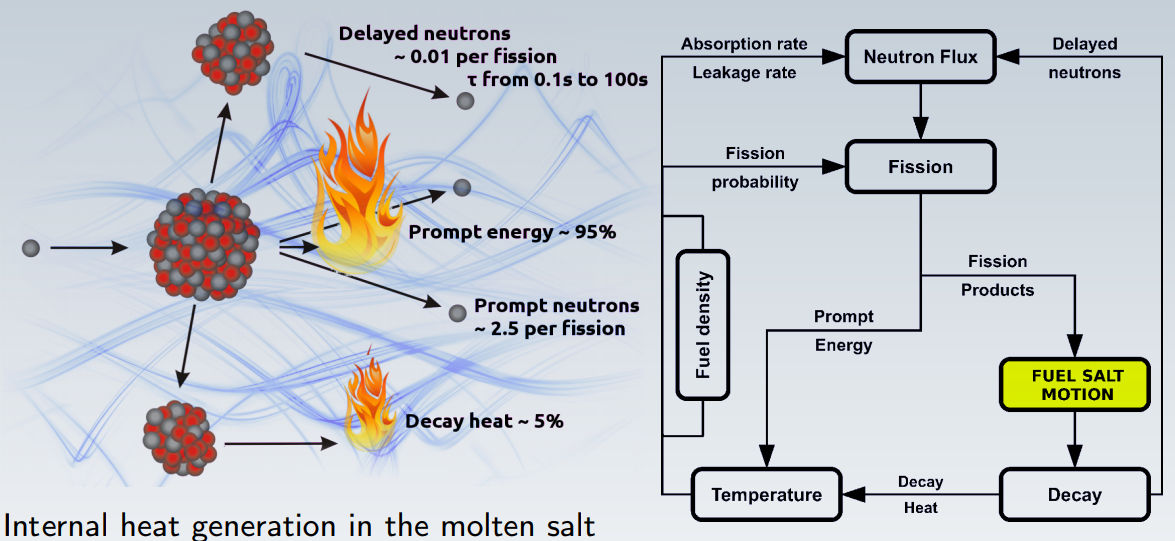
\includegraphics[height=0.47\textwidth]{./images/coupled_physics.png}
		\vspace*{-0.05in}
		\caption{Challenges in simulating \glspl{MSR} (Image courtesy of Manuele Aufiero,2012).}
     	 \end{figure}               
\end{frame}

\begin{frame}
  \frametitle{Research objectives}
                  \vspace*{-0.1in}

              \begin{block}{Multiphysics simulation of \gls{MSR} (Moltres/MOOSE)\cite{lindsay_introduction_2018}}
               \begin{enumerate}
                \item Demonstrate steady-state and transient coupling of neutron fluxes, precursor drift, and thermal-hydraulics
                \item Implement advective movement of delayed neutron precursors
                \item Demonstrate capabilities with 2D axisymmetric and 3D mesh
                \item Simple transients: change of flow and moderator movement
               \end{enumerate}
               \end{block}


              
\end{frame}
